\section{Biological response to ENSO variability}

\subsection{Mean state}

Before analysing the biological response of fish biomass to ENSO variability, the mean state of the Apecosm model will be investigated.
For the sake of simplicity, the focus will be laid on three size classes: 2 cm, representing small fishes, 20cm, representing intermediate sizes, and 90 cm, representing large individuals. These sizes are also
representative of the sizes of tuna target species within the region.
\warn{ref!!!}.  \\ 

Figure \ref{fig:mean-cov-ape} shows the mean fish-biomass density ($J.m^{-2}$) for the three different size-classes.
\warn{interpret these figures}

\begin{figure}[h!]
    \centering
    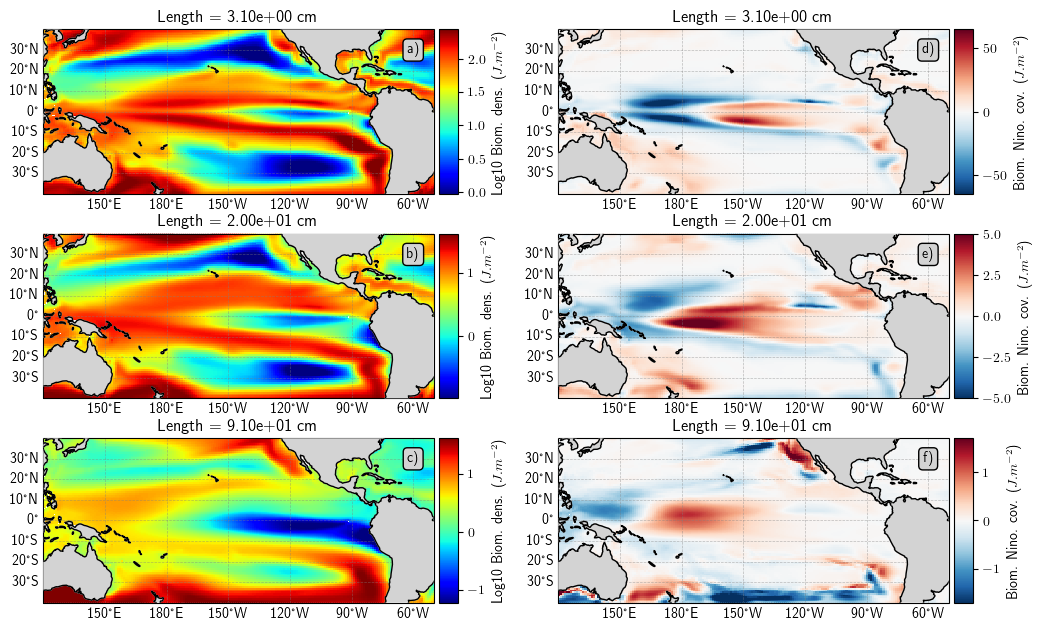
\includegraphics[width=\textwidth]{covariance_mean_epi.png}
    \caption{Yearly average of biomass density (left panel, log-scale, $J.m^{-2}$) and 
    covariance between the yearly average biomass density and the winter-average ONI index (right panels, $J.m^{-2}$)}
    \label{fig:mean-cov-ape}
\end{figure}

\subsection{Interannual response to ENSO variability}

In order to investigate the response of fish biomass to ENSO variability, the methodology described in section \ref{sec:pisces} has been applied on the vertically integrated fish biomass density ($J.m^{-2}$). The covariance maps are shown in figure \ref{fig:mean-cov-ape} for the three sizes. 

Small epipelagics show negative anomalies shows negative anomalies at around 5N and 5S, and shows slightly positive anomalies 
near the equator. Intermediate epipelagics show positive anomalies in the central Pacific and negative ones in the west.
The pattern for large epipelagics is similar to that of intermediate sizes, although the positive anomalies are weaker and shifted westward.\\

\subsection{Transient biological response to \nino}

\begin{figure}[h!]
    \centering
    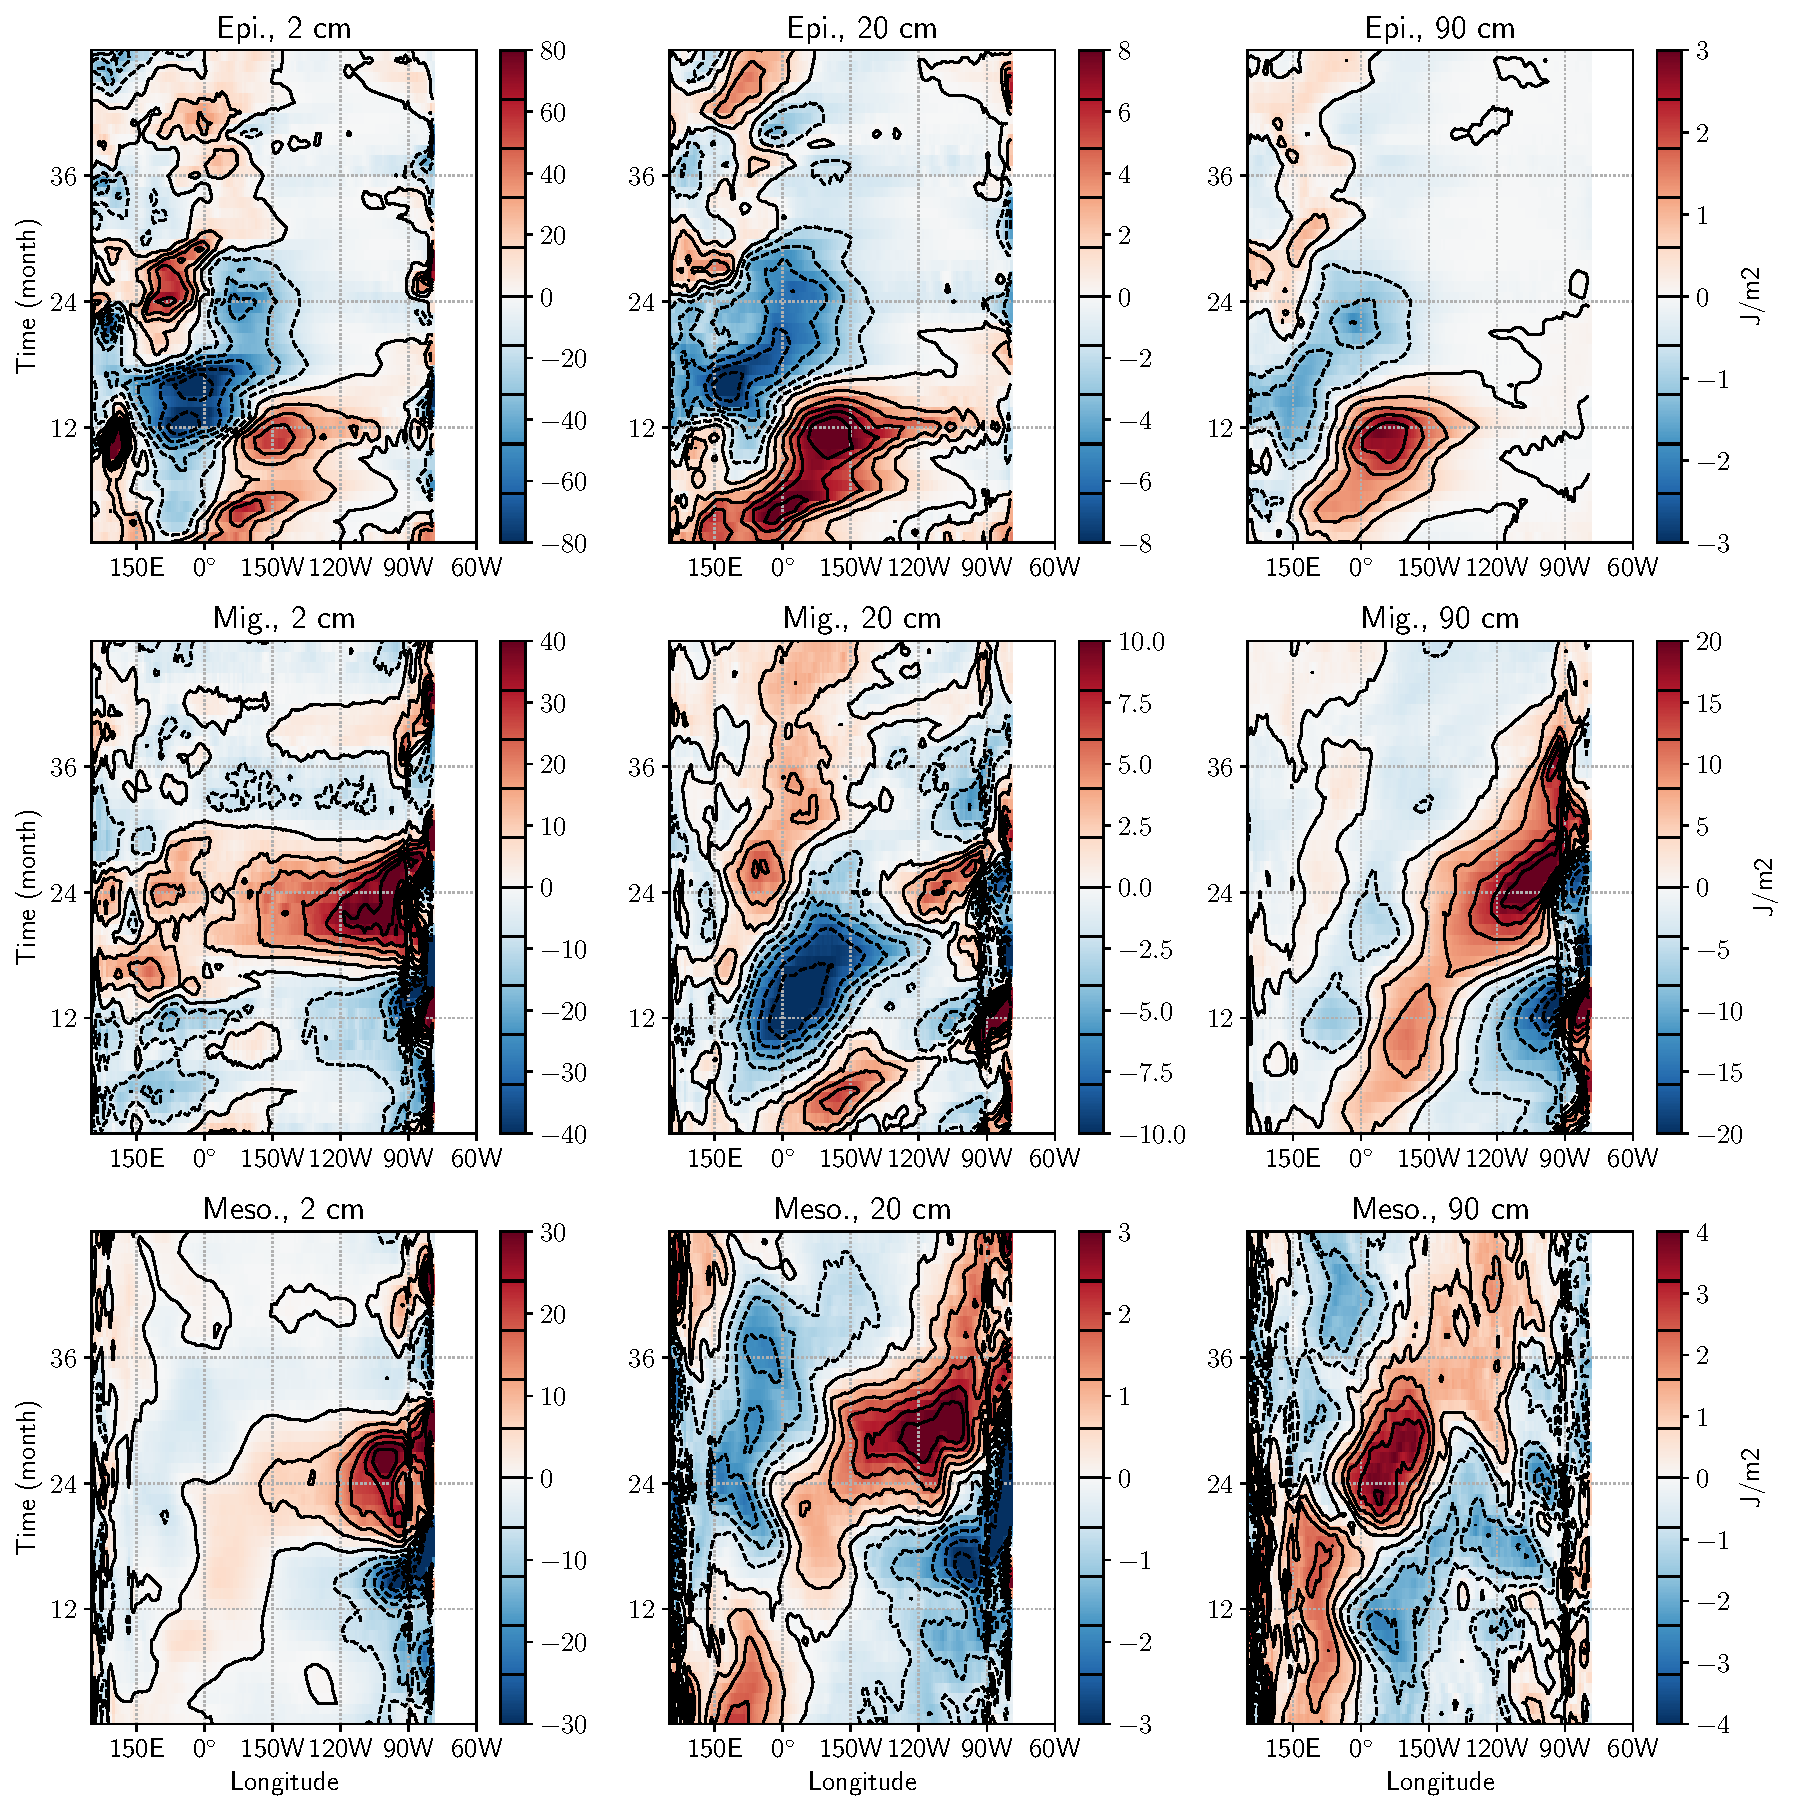
\includegraphics[scale=0.5] {debugged_corr_mask_hovmoller_composites_OOPE}
    \caption{Composites of \hov\ diagram composite of fish biomass density ($J.m^{-2}$) along the equatorial Pacific ocean.}
    \label{fig:hov-oope}
\end{figure}

\clearpage
